\chapter{Experiments based on Ohm's Law}
	\section{Aim}
		\begin{itemize}
			\tightlist
			\item Explain Ohm's Law
			\item Explain Ohm's Law for Resistance in series
			\item Explain Ohm's Law for Resistance in parallel
			\item Explain Non-Ohmic Device
			\item Measure and confirm Ohm's Law
		\end{itemize}

	\section{Apparatus}
		Ammeter, Voltmeter, Resistors, Battery, Wires
		
	\section{Theory}
		\subsection{Ohm's Law}
			\begin{enumerate}
				\item The law states that the current through a conductor between two points is directly proportional to the voltage across the two points. Such a conductor is characterized by its ‘Resistance’ – $R$ measured in Ohms.
				\item $V = IR$
					\begin{itemize}
						\tightlist
						\item $V$ is the Voltage in Volts across the conductor.
						\item $I$ is the current in Amperes through the conductor.
						\item Voltage($V$) is directly proportional to current($I$) i.e. $V \propto I$
						\item Resistance($R$) in inversely proportional to current($I$) i.e. $I \propto R$
					\end{itemize}
			\end{enumerate}
		
		\subsection{Explanation of Ohm's Law}
			\begin{figure}[h]
				\centering
				\includegraphics[width=0.5\linewidth]{img/exp4/1}
				\caption{Current Through Resistor}
				\label{fig:currentThroughResistor}
			\end{figure}
			From the circuit:
			
			The voltage across resistor is equal to source voltage:
			$$V_R=V_S$$
			The current through the resistance is given by:
			$$I=\frac{V_R}{R}$$
		
		\subsection{Explaination of Ohm's Law for Resistance in series}
			Series circuits are sometimes called current-coupled or daisy chain-coupled. The current in a series circuit goes through every component in the circuit. Therefore, all of the components in a series connection carry the same current. There is only one path in a series circuit in which the current can flow.
			
			Current:
			$$I=I_1=I_2=I_3$$
			Resistance:
			$$R_{eq}=R_1+R_2+R_3$$
			Voltage:
			$$V_S=V_{R1}+V_{R2}+V_{R3}$$
			\begin{figure}[h]
				\centering
				\includegraphics[width=0.5\linewidth]{img/exp4/2}
				\caption{Series Resistors}
				\label{fig:seriesResistors}
			\end{figure}
		
			From the circuit:
			
			The equivalent resistance,
			$$R_{eq}=R_1+R_2$$
			The total current of the circuit,
			$$I_T=\frac{V_S}{R_{eq}}$$
			Voltage across each resistance are,
			For resistance \(R_1\),
			$$V_{R1}=R_1 \times I_T$$
			For resistance \(R_2\),
			$$V_{R2}=R_2 \times I_T$$
			
			In a series circuit, the current through each of the resistors is the same, and the voltage across the circuit is the sum of the voltages across each resistor.
			
		\subsection{Explaination of Ohm's Law for Resistance in parallel}
			If two or more components are connected in parallel they have the same potential difference (voltage) across their ends. The potential differences across the components are the same in magnitude, and they also have identical polarities. The same voltage is applicable to all circuit components connected in parallel. The total current is the sum of the currents through the individual components, in accordance with Kirchhoff’s current law.
			
			Voltage:
			$$V=V_1=V_2=V_3$$
			Resistance:
			$$\frac{1}{R_{eq}}=\frac{1}{R_1}+\frac{1}{R_2}+\frac{1}{R_3}$$
			Current:
			$$I_T=I_{R1}+I_{R2}+I_{R3}$$
			\begin{figure}[h]
				\centering
				\includegraphics[width=0.5\linewidth]{img/exp4/3}
				\caption{Parallel Resistors}
				\label{fig:parallelResistors}
			\end{figure}
		
			From the circuit:
			
			The equivalent resistance,
			$$ R_{eq}=\frac{R_1 \times R_2}{R_1+R_2}$$
			The total current of the circuit,
			$$I_T=\frac{V_S}{R_{eq}}$$
			Current across each resistance are,
			For resistance \(R_1\),
			$$ I_{R1}=\frac{V_S}{R_1}$$
			For resistance \(R_2\),
			$$ I_{R2}=\frac{V_S}{R_2}$$
			
			In a parallel circuit, the voltage across each of the resistors is the same, and the total current is the sum of the currents through each resistor.
			
		\subsection{Explaination of Non-Ohmic Device}
			A Non ohmic device is a device that does not obey Ohm's Law i.e. the resistance is not constant, but changes in a way that depends on the voltage across it.The device is said to be non-Ohmic. In this case V versus I graph is not a straight line, but has some curvy shape. Such devices do not have a constant value of resistance and the resistance is called dynamic resistance because it is constantly changing.Examples of such devices are tungsten filament (bulb), diode,thermistor etc.
			\begin{figure}[h]
				\centering
				\includegraphics[width=0.5\linewidth]{img/exp4/4}
				\caption{Non-Ohmic Devices}
				\label{fig:nonOhmicDevices}
			\end{figure}
			
	\section{Procedure}
		\subsection{Experiment of confirming Ohm's Law}			
			\begin{enumerate}
				\tightlist
				\item
				Set DC voltage $0-30V$.
				\item
				Set the Resistance Value $(1 K\Omega - 100 K\Omega)$.
				\item
				Voltmeter is placed parallel to resistor and ammeter series with
				resistor.
				\item
				Now note the Voltmeter and Ammeter reading for DC voltage.
				\item
				Increase the DC voltage by 2 factor and note Voltmeter and Ammeter
				Readings. Keep resistance value constant
				\begin{figure}[h]
					\centering
					\includegraphics[width=0.4\linewidth]{img/exp4/5}
					\caption{}
					\label{fig:exp4_1}
				\end{figure}
				\item
				Plot the $V-I$ graph to verify Ohm's Law.
				\item
				Repeat step 2 to 6 for another set of resistance value.
				\item
				$V$ versus $I$ graph is a straight line.
				\item
				Therefore from the graph we see that the resistance do adhere to Ohm's
				law. Thus resistance is said to be an Ohmic device.
			\end{enumerate}
		
		\subsection{Experiment with Resistance in series}				
			\begin{enumerate}
				\tightlist
				\item
				Set DC voltage $0-30 V$.
				\item
				Here resistance are kept in series. Set the resistance $R_1 (1 K\Omega - 100
				K\Omega)$ value and set resistance $R_2 (5K\Omega - 15K\Omega)$.
				\item
				Voltmeter is placed parallel with resistor and ammeter series with
				resistor.
				\item
				Now note the Voltmeter and Ammeter reading for DC voltage.
				\begin{figure}[h]
					\centering
					\includegraphics[width=0.4\linewidth]{img/exp4/6}
					\caption{}
					\label{fig:exp4_2}
				\end{figure}
				\item
				Increase the DC voltage by 2 factor and note Voltmeter and Ammeter
				Readings. Keeping resistance value constant
				\item
				Plot the $V-I$ graph to verify Ohm's Law
				\item
				Repeat step 2 to 6 for another set of resistance value.
			\end{enumerate}
		
		\subsection{Experiment with Resistance in parallel}
			\begin{enumerate}
				\tightlist
				\item
				Set DC voltage $0-30 V$.
				\begin{figure}[h]
					\centering
					\includegraphics[width=0.4\linewidth]{img/exp4/7}
					\caption{}
					\label{fig:exp4_3}
				\end{figure}
				\item
				Here Resistances are kept parallelly. Set the resistance $R_1 (100\Omega-
				2K\Omega)$ value and set resistance $R_2(1K\Omega -30K\Omega)$.
				\item
				Voltmeter is placed parallel to resistor and ammeter series with
				resistor.
				\item
				Now note the Voltmeter and Ammeter reading for DC voltage.				
				\item
				Increase the DC voltage by 2 factor and note Voltmeter and Ammeter
				Readings. Keeping Resistance value constant
				\item
				Plot the $V-I$ graph to verify Ohm's Law.
				\item
				Repeat step 2 to 6 for another set of resistance value.
			\end{enumerate}

		\subsection{Experiment with Non-Ohmic Device}
			\begin{enumerate}
				\tightlist
				\item
				Set DC voltage to $5V$.
				\item
				Use the resistor of $100K\Omega$ and a diode.
				\item
				Voltmeter is placed parallel to Silicon diode and ammeter series with
				resistor.
				\item
				Now note the Voltmeter and Ammeter reading for DC voltage $5V$.
				\begin{figure}[h]
					\centering
					\includegraphics[width=0.4\linewidth]{img/exp4/8}
					\caption{}
					\label{fig:exp4_4}
				\end{figure}
				\item
				Decrease the Resistance as $75K\Omega$, $51K\Omega$, $24K\Omega$ and $10K\Omega$ and take the
				readings and note Voltmeter reading across Silicon diode and Ammeter
				reading.
				\item
				Plot the $V-I$ graph and observe the change.
				\item
				The Change is not simply proportional. $V$ versus $I$ graph is not a
				straight line.
				\item
				Therefore from the graph we see that the diode does not adhere to Ohms
				law.Thus diode is said to be non-Ohmic device.
			\end{enumerate}

	\section{Observations}
		\begin{figure}[h]
			\centering
			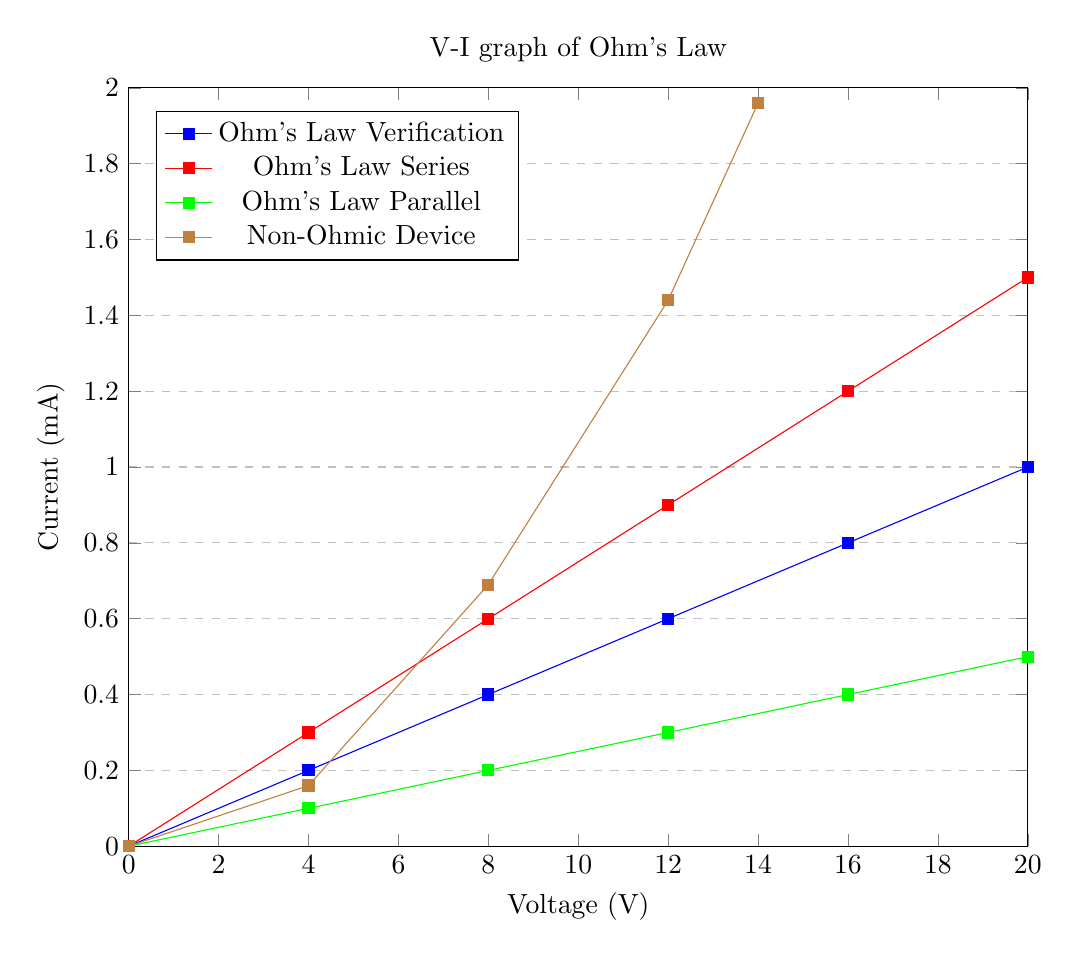
\begin{tikzpicture}
				\begin{axis}[
					title={V-I graph of Ohm's Law},
					width=13cm,
					xlabel={Voltage (V)},
					ylabel={Current (mA)},
					xmin=0, xmax=20,
					ymin=0, ymax=2,
					xtick={0,2,4,6,8,10,12,14,16,18,20},
					ytick={0,0.2,0.4,0.6,0.8,1.0,1.2,1.4,1.6,1.8,2.0},
					legend pos=north west,
					ymajorgrids=true,
					grid style=dashed,
					legend entries = {Ohm's Law Verification,Ohm's Law Series,Ohm's Law Parallel,Non-Ohmic Device}
					]
					
					\addplot[
					color=blue,
					mark=square*,
					]
					coordinates {
						(0,0)(4,0.2)(8,0.4)(12,0.6)(16,0.8)(20,1)
					};
					
					\addplot[
					color=red,
					mark=square*,
					]
					coordinates {
						(0,0)(4,0.3)(8,0.6)(12,0.9)(16,1.2)(20,1.5)
					};
				
					\addplot[
					color=green,
					mark=square*,
					]
					coordinates {
						(0,0)(4,0.1)(8,0.2)(12,0.3)(16,0.4)(20,0.5)
					};
					
					\addplot[
					color=brown,
					mark=square*,
					]
					coordinates {
						(0,0)(4,0.16)(8,0.69)(12,1.44)(14,1.96)
					};
					
				\end{axis}
			\end{tikzpicture}
			\caption{Observation $V-I$ Graph}
		\end{figure}
		\begin{figure}[h!]
			\begin{longtable}[]{@{}llllll@{}}
				\toprule
				Sr No. & Voltage(V) & Ohm's Exp (I) & Series (I mA) & Parallel (I mA) & Non-Ohmic (I mA)\tabularnewline
				\midrule
				\endhead
				1 & 0 & 0 & 0 & 0 & 0\tabularnewline
				2 & 4 & 0.2 & 0.3 & 0.1 & 0.16\tabularnewline
				3 & 8 & 0.4 & 0.6 & 0.2 & 0.69\tabularnewline
				4 & 12 & 0.6 & 0.9 & 0.3 & 1.44\tabularnewline
				5 & 16 & 0.8 & 1.2 & 0.4 & 2.56\tabularnewline
				6 & 20 & 1 & 1.5 & 0.5 & 4\tabularnewline
				\bottomrule
			\end{longtable}
			\caption{Observation Values}
		\end{figure}
	
	\section{Result}
		V versus I graph is a straight line. Which means voltage is directly proportional to
		current. Therefore, Ohm’s law is verified for Ohmic-devices.